
\chapter{Description of the GAMMA-400 prototype detector}
\label{cap:experiment}
%
%To develop and test new detector, a well established reference has to be
%defined. Since 2007 the reference tracking system used in the INSULAB group is the
%so-called {\em INSULAB Telecope}
%
%. It has been originally 
%developed for the for the COHERENT experiment~\cite{Hasan:1353904,Lietti201284}
%to study with.



\section{{\color{red}The AGILE and FERMI experiments}}
\label{sec:agile_fermi}

\section{The GAMMA-400 instrument}
\label{sec:gamma400}
The \gls{gamma} space observatory is a space mission founded by the Russian
Space Agency aimed to investigate aspect of gamma ray astronomy, cosmic ray
science and high energy charged particle spectra measurement. The \gls{gamma}
experiment will be hosted on the {\em Navigator} space platform, which is able
to accommodate high mass and large volume scientific payload. The use of the
{\em Navigator} opens new solution to space experiments, since it allows the
installation of heavy devices, with relatively large energy requirements. It
also provides a broad downlink band ($\sim$100 GB/day). Due to these unique
features it is expected to significantly contribute to the next generation of
space instruments for gamma ray astronomy and cosmic ray physics.\\
The \gls{gamma} apparatus~\cite{Galper:2011bc} consists of a gamma ray
telescope, two star sensors with 5 arc-second accuracy, a gamma ray burst
monitor (the KONUS- FG)~\cite{Aptekar:2009sk}, four direction detectors located
on telescopic
booms, two spectrometric detectors and two magnetometers.\\
Among the original goals of the mission:
\begin{itemize}
\item the study of unidentified gamma-ray sources, which are one third of
  discovered gamma-ray sources;
\item a detailed investigation of the Galactic center;
\item study sources where the energy ranges of Fermi and ground-based gamma ray telescopes do not overlap
\item search for high energy emission from gamma ray bursts and transient
  gamma ray sources;
\item search for a fine structure in the spectra of high energy cosmic ray
  electron-positron and nuclei.
\end{itemize}
Moreover, the measurements in the gamma ray spectra in the region near 100~GeV
showed some discrepancies between the result obtained by Fermi and ground-based
telescopes. This energy region is therefore of huge interest, because diffuse
gamma ray emission above 100~GeV can provide hints to the origin of the dark
matter. A candidate is in fact a 135~GeV right-handed neutrino, suggested by a
gamma ray differential energy spectrum analysis~\cite{Bergstrom:2012bd}.\\
The original design of the instrument, whose proposal dates back the late
80's~\cite{Dogiel1989} has been improved~\cite{Galper:2011bc} using the result
of Fermi and AGILE missions. In recent years, the collaboration between Italian
and Russian groups has result in a significant improvement of the apparatus
performances. \fig{fig:gamma400} is a schematic view of the telescope.
\begin{figure}[!htbp]
\centering
\includegraphics[width=.4\textwidth]{immagini/gamma400_design.jpg}
\caption{\small \it Physical scheme of the GAMMA-400 telescope.}\label{fig:gamma400}
\end{figure}
It consists of
\begin{itemize}
\item an anti-coincidence system (AC), whose goal is discriminate between charged
  and neutral particles. It is located both on top and on the lateral side of
  the telescope, and is composed by plastic scintillator read out withSiliconPhotomultipliers;
\item a converter-tracker system (C), used to convert photons into $e^+-e^-$
  pairs and to precisely reconstruct the photon direction.  It consists of 10
  double layers of microstrip silicon detectors, interleaved with 0.08 X$_0$ thick tungsten
  layers;
\item a \gls{tof} system used both to generate the trigger for the telescope and
  to reject albedo particles by measuring their velocity. It consists of plastic
  scintlllators coupled to Silicon Photomultiplier;
\item a shallow imaging calorimeter (CC1) composed by 2 layers of CsI(Tl)
  crystals interleaved with 2 silicon microstrip layers, of the same type used
  for the converter-tracker system. The calorimeter, 1X$_0$ deep is finely
  segmented so that it can precisely measure each converted $e^+-e^-$ pair after
  a large 50 cm lever arm below the converter-tracker. It results in a
  significant improvement of the photon angular resolution;
\item a deep, isotropic, homogeneous calorimeter (CC2) that allow optimal
  detection of high energy hadrons up to $10^{15}$ eV. It is composed by 28$\times$28$\times$12
  cubic CsI(Tl) crystals with 3.6 cm side developed on the basis of the CaloCube
  project~\cite{Adriani:2013mya}. 
\item a neutron detector (ND), located below the CC2, whose goal is to improve the proton/electron ratio.
\end{itemize}

The converter-tracker system is assembled in 4 towers, each 50$\times$50
cm$^2$. The silicon miscrostrip detectors are arranged in ladders, 50 cm long,
readout at their ends.  The present design of the silicon microstrip sensors
foresees single sided devices with an implant pitch of 80 $\mu$m and a readout
pitch of 240 $\mu$m; this readout scheme was chosen in order to reduce as much
as possible the number of electronic channels. A good good spatial resolution is
achieved making use of the capacitive charge division
approach~\cite{KOTZ1985481}.  In this configuration the Si-W tracker features an
overall number of 2000 silicon sensors and 153600 readout channels. Thanks to
the use of low-power ASICs, the total power consumption of the tracker front-end
electronics is approximately 80 W~\cite{Galper:2011bc}.\\
The overall dimensions of the CC2 calorimeter (1$\times$1$\times$ 0.47 m$^3$)
correspond to 54.6$\times$54.6$\times$23.4 radiation lengths, and allow the
containment of particles up to $\sim$10 TeV. In addition to this the overall
mass of $\sim$2000 kg provides an effective geometric factor of the order of
4m$^2$sr that is the key for the detection of high energy hadrons, giving the
possibility to directly probe on orbit the knee region. The significant overall
geometric factor increment is achieved detecting the particles not only on the
top surface but also on the lateral side.\\

Gamma rays are detected via the conversion into electron-positron pair in the
converter-tracker system. The direction of the incoming particle is determined
using the \gls{tof} system, where the detectors S1 and S2 are 500mm apart each
other. The silicon microstrip detector, together with the anti-coincidence
detectors located at front and sides of the converter-tracker allow to identify
gamma rays. The electromagnetic cascade initiated with the electron-positron
pair develops in the CC1 and CC2 calorimeters.  The combination of the tracking
system and the position sensitive calorimeter CC1, permits the reconstruction of
the electromagnetic cascade axis, provide a high angular resolution. This
combination allows to reach the superior angular resolution of
$\sim\ang{0.01}$ above 100 GeV. Informations from the calorimeters together
with the additional scintillation detectors S3 and S4 that can detect cascade
particles provides a energy resolution up to $\sim$1\% above 100 GeV. Electrons,
positrons and nuclei can be detected when coming from the lateral directions as
well. In this case particles are detected using the lateral detectors, and their
charge is determined using the two silicon arrays at the top and in the middle
of the assembly.\\

The \gls{gamma} telescope basic parameters are presented
in~\tab{tab:gamma400_info}, while~\tab{tab:gamma400_comparison} shows a
comparison between space-based and ground-based instruments:
EGRET~\cite{Thompson:1993zz}, AGILE~\cite{Tavani:2008sp},
Fermi~\cite{Abdo:2009gy}, CALET~\cite{Torii:2008zz},
H.E.S.S.~\cite{Aharonian:2005kn}, MAGIC~\cite{Aleksic:2011bx}, 
VERITAS~\cite{Weekes:2010zz}
 and CTA~\cite{Medina:2011be}
\begin{table}[!htb]
  \begin{center}
    \begin{tabular}{|l|l|}\hline
      Energy range & 100 MeV - 3000 GeV\\
      Field-of-view, sr (E$_\gamma$ > 1 GeV) & $\sim$ 1.2\\
      Effective area, cm$^2$ (E$_\gamma$ > 1 GeV) & $\sim$ 4000\\
      Energy resolution (E$_\gamma$ > 10 GeV) & $\sim$ 1\%\\
      Angular resolution (E$_\gamma$ > 100 GeV) & $\sim$ $0.01\si{\degree}$\\
      Converter-tracker thickness & $\sim$ 1 X0\\
      Calorimeter thickness & $\sim$25 X0\\
      Proton rejection factor & $\sim$ 106\\
      Telemetry downlink volume, Gbyte/day & 100\\
      Total mass, kg & 2600\\
      Maximum dimensions, m$^3$ & 2.0$\times$2.0$\times$3.0\\
      Power consumption, W & 2000\\
\hline
    \end{tabular}
    \caption{aa}\label{tab:gamma400_info}
  \end{center}
\end{table}
\begin{table}[!tb]
\begin{center}
\resizebox{\textwidth}{!}{%
\begin{tabular}{l|lllll|llll}
\hline
 & \multicolumn{5}{c}{Space-based} & \multicolumn{4}{c}{Ground-based} \\
 \hline
& EGRET & AGILE & Fermi -LAT & CALET & GAMMA-400 & H.E.S.S. & MAGIC & VERITAS & CTA\\
Energy range (GeV) & 0.03-30 & 0.03-50 & 0.1 - 300 & 10-10000 & 0.1 - 3000 & >100 & >50 & >100 & >10\\
\begin{tabular}{@{}l}Angular resolution (deg)\\{\tiny E$_\gamma$ > 100 GeV}\end{tabular} & \begin{tabular}{@{}l}0.5\\{\tiny E$_\gamma$ 10 GeV}\end{tabular} & \begin{tabular}{@{}l}0.1\\ {\tiny E$_\gamma$ 1 GeV}\end{tabular} & 0.05 & 0.1 & 0.01 & 0.2 & 0.1 & 0.1 & 0.1\\
\begin{tabular}{@{}l}Energy resolution (\%)\\{\tiny E$_\gamma$ > 100
  GeV}\end{tabular} & \begin{tabular}{@{}l}20\\{\tiny E$_\gamma$ < 10
                        GeV}\end{tabular} & \begin{tabular}{@{}l}50\\{\tiny
                                              E$_\gamma$ < 10 GeV}\end{tabular}
 & 10 & 2 & 1 & 20 & 12 & 10 & 15\\
\hline
\end{tabular}
}
\caption{aa}\label{tab:gamma400_comparison}
\end{center}
\end{table}
A detailed comparison between \gls{gamma} and Fermi-LAT can be found in~\cite{Galper:2014pua}.


\section{The GAMMA-400 prototype silicon sensors}
In order to explore different solution in terms of sensor features a \gls{gamma}
prototype silicon sensors, characterized by different zones with different
implant widths and readout schemes has been used. The prototype sensors have
been manufactured at the \gls{cmm}, FBK, Trento (Italy)~\cite{cmm-fbk}. The sensors have
been built using high-resistivity, high-purity n-type silicon wafers of 6
in diameter.\\
The detectors have a dimension of 53.16$\times$32.76 mm$^2$ and a
thickness of 300 $\mu$m. Two solutions for the sensor layout have been
adopted:
\begin{itemize}
\item the first sensor has a p+ implant made of 384 strip with pitch of 80
  $\mu$m;
\item the second has a p+ implant made of 256 strip with pitch of 120
  $\mu$m.
\end{itemize}
In both designs, the strips are AC-coupled via integrated coupling capacitors
and the DC-bias of the strips is achieved by punch-through.\\
Both the sensors are further divided into different zones, each characterised
with different features in term of strip pitch and implant width.
\begin{itemize}
\item in the 80 $\mu$m pitch sensor 6 groups of 64 strips each are
  present. Implants width are 20, 30, 40, 50, 55 and 60 $\mu$m;
\item in the 120 $\mu$m pitch sensors the strips are divided in 4 groups of 64
  strip each. Implants width are 30, 40, 50 and 60 $\mu$m.
\end{itemize}
\tab{tab:basculo_features} summarises the features of each zone of the two
sensors, with emphasis on the physical and readout pitch.
\begin{table}[!htb]
\begin{center}
\resizebox{.7\textwidth}{!}{%
\begin{tabular}{rrrrr}
\hline
\myalign{c}{zone} & \myalign{c}{physical pitch}& \myalign{c}{readout pitch}& \myalign{c}{implant width}
& \myalign{c}{number of ASIC}\\
& \myalign{c}{($\mu$m)} & \myalign{c}{($\mu$m)} & \myalign{c}{($\mu$m)}
& \myalign{c}{channels}\\
\hline
1     & 120     & 	120  &   30  &    18    \\
2     & 120     & 	240  &   30  &    16    \\
3     & 120     & 	240  &   40  &    17    \\
4     & 120     & 	120  &   40  &    15    \\
5     & 120     & 	120  &   50  &    17    \\
6     & 120     & 	240  &   50  &    14    \\
7     & 120     & 	240  &   60  &    16    \\
8     & 120     & 	120  &   60  &    17    \\
9     &   80    & 	160  &   20  &    14    \\
10    &   80    & 	240  &   20  &    10    \\
11    &   80    & 	240  &   30  &    10    \\
12    &   80    & 	160  &   30  &    10    \\
13    &   80    & 	160  &   40  &    11    \\
14    &   80    & 	240  &   40  &    12    \\
15    &   80    & 	240  &   50  &    9     \\
16    &   80    & 	160  &   50  &    13    \\
17    &   80    & 	160  &   55  &    10    \\
18    &   80    & 	240  &   55  &    10    \\
19    &   80    & 	240  &   60  &    9     \\
20    & 80      & 	160  &   60  &    19    \\
\hline
\end{tabular}
}
\caption{\small\it The GAMMA-400 detector prototype is built using two different
  sensors, each characterised by different physical and readout pitch, implant
  width and numer of ASIC channels.}\label{tab:basculo_features}
\end{center}
\end{table}
\fig{fig:basculo_schema} is a schematic representation of the prototype that
shows how the sensors and zones are displaced. The final assembly is depicted in
\fig{fig:basculo_img}.
\begin{figure}[!htb]
\centering
\subfloat[] {
  \includegraphics[width=.4\textwidth]{immagini/basculo_layout.png}\label{fig:basculo_schema}
}
\subfloat[] {
  \includegraphics[width=.4\textwidth]{immagini/basculo.png}\label{fig:basculo_img}
}
\caption{\small \it Schematic of the displacement of the different zones (a) in the
  two sensors and picture of the final assembly (b).}\label{fig:basculo}
\end{figure}

The readout electronic is composed of five VA140 \gls{asic}s built in 0.35
$\mu$m CMOS technology. VA140~\cite{va140} is a 64 channel low noise/low power charge
sensitive preamplifier-shaper circuit with high dynamic range ($\pm$200 fC). It
features simultaneous sample and hold, multiplexed analogue readout, calibration
facilities and internally generated biases. \tab{tab:asic_basculo} describes its
main features.\\

\begin{table}[!htb]
\begin{center}
\resizebox{.7\textwidth}{!}{%
\begin{tabular}{ll}
\hline
Number of inputs &	64\\
Input charge range	& $\pm$200 fC \\
Shaping time	& 5 - 8 $\mu$s \\
Nominal capacitive load	& 50 pF \\
Equivalent Noise Charge	& 98e + 6.5e/pF\\
Outputs &	Multiplexed pulse height\\
Test and calibration &	Internal calibration circuit\\
Power consumption	& 0.29 mW/channel\\
\hline
\end{tabular}
}
\caption{\small\it Features of the VA140 ASIC.}\label{tab:asic_basculo}
\end{center}
\end{table}

To further explore viable configurations the detectors are placed in an
aluminium frame interfaced with a tiltable support that allows to measure the
spatial resolution for different angles of the incoming particles. The tilt
angle can be selected in steps of 15$\si{\degree}$, inserting a calibrated metal
pin in a drilled wheel. The aluminum frame also provides protection for the
sensors and holds the front-end electronics.\\
The GAMMA-400 prototypes were tested on the CERN T9 beamline~(\sect{sect:t9beamline}), using negative
particles (mainly muons and pions) with an energy of 10 GeV. In the experimental
setup the \gls{gamma} prototype detector was placed between two modules of the
INSUBLAB Telescope (see~\sect{sect:telescope} for a detailed description) to obtain a tracking system. The chosen modules are
manifactured by CSEM\footnote{Centre Suisse dElectronique et de Microtechnique
  SA, CH, http://www.csem. ch/site/} and readout by three VA2 128 channel ASICs,
built with a 1.2 $\mu$m N-well CMOS technology. A representation of
the assembly is shown in~\fig{fig:gamma400_final_assembly}.\\
\begin{figure}[!htb]
\centering
  \includegraphics[width=.4\textwidth]{}
\caption{\small \it Schematic of the tracking system assembly.}\label{fig:gamma400_final_assembly}
\end{figure}

The system is triggered by two scintillator counters: 
\begin{itemize}
\item a first scintillator, whose area is 10$\times$10 cm$^2$ is positioned
  directly at the end of the beamline;
\item a second scintillator of area 3$\times$4, hence of smaller dimension, is directly mounted on the first silicon telescope by means of a dedicated support.
\end{itemize}

The DAQ is a standard VME system controlled by a SBS Bit3 model 620 bridge2,
optically linked to a Linux PC-system. 

The trigger signal is generated by a custom VME board (the trigger board) when a
coincidence of the who scintillator counters and the spill signal occurs. The
trigger signal is then sent to three VME VRB boards~\cite{Berra2014422} designed
by INFN-Trieste to generate the DAQ trigger and the readout sequence of the
silicon detectors; the VRB boards are also responsible for the ASICs
configuration before the start of the run.\\
The VRB hosts an Altera EP2C50 FPGA with 50k cells and 581kbit of internal RAM
(which allows also to check complex designs with the embedded logic state
analyzer) and 4 PLLs (Phase Locked Loop) for the clock generation. The board has
16 LVDS (Low-Voltage Differential Signaling) inputs and 16 LVDS outputs, 2 TTL
inputs and 2 TTL outputs, a TLK1501 Gigabit link and 4 Mword of 32 bit RAM. When
the VRB receives the data, the input from each board is de-multiplexed and each
stream of data is copied in the RAM, and transferred to the PC during the
interspill period.\\
The signals of both the silicon beam telescopes and of the GAMMA-400 prototype
are digitised by three dedicated ADC boards and sent back to the control
boards.\\

Since the \gls{gamma} prototype dimensions exceed the telescope modules
dimensions, data taking have required different runs for the complete scan of
the board. Moreover, five different tilt angle configurations between
-15\si{\degree} and 60\si{\degree} were tested.


\section{The INSULAB telescope}\label{sec:telescope}
Since 2007 the INSULAB group has provided a silicon-based tracking system, the
{\em INSULAB Telecope}, for different INFN projects:
\begin{itemize}
\item very accurate studies of the deflection and radiation properties of bent
  crystals of a large variety of materials (Si, Ge, SiGe graded, LiNbO3,
  \ldots)~\cite{bagli-coherent,desalvador-ge_crystals}, types (quasimosaic,
  single- or multi-strip~\cite{Hasan:1353904}) and dimensions from hundreds of $\mu$m
  down to tens of nm along the beam direction~\cite{Mazzolari2013130} for the NTA-HCCC3,
  COHERENT4 and ICE-RAD5 experiments~\cite{Hasan:1353904,Lietti201284};
\item studies of large area and large dynamic range Silicon PhotoMultipliers
  (SiPMs) for high energy and space physics, in particular coupled to shashlik
  or LYSO/PbWO4 crystal based electromagnetic calorimeters (the FACTOR6 and
  TWICE7 projects~\cite{Berra:1458946,Berra2013380,guffanti-LYSO}).
\end{itemize}
The original tracking system, based on~\cite{Celano199649}, has been developed
by INFN-Ts and used to test the BaBar SVD
prototype~\cite{bari1996results}. During the years many modules have been added
to the system to test different solutions and to increase the performances of
the instrument limiting the material along the beamline. One of the main reason
of the system improvement was the availability of self triggering ASICs, that
allowed the assembly of a very compact silicon only system.\\
The INSULAB Telescope consistes of different modules, equipped with silicon
microstrip detectors manufactured by three producers (single side ones by
HAMAMATSU\footnote{HAMAMATSU Photonics, \url{www.hamamatsu.com}.} and double
side ones by FBK-irst\footnote{Fondazione Bruno Kessler, \url{www.fbk.eu}} and
CSEM\footnote{Centre Suisse d'Electronique et Microtechnique Neuchatel, \url{www.
csem.ch}.}) and different readout electronics (VA2~\cite{va2_spec},
VA1 prime2~\cite{va1prime_spec} and VA1TA~\cite{va1ta_spec} by IDEAS). The main
features of the telescope are summarised in~\tab{tab:telescope}.
\begin{center}
\begin{table}
\resizebox{\textwidth}{!}{%
  \begin{tabular}{l | llll}
\hline
    Detector & Double & Double & Double (only \(\Omega\)) & Single\\
    Produced by & CSEM & FBK-IRST & FBK-IRST & HAMAMATSU\\
    ASIC & VA2 & VA1\(_{\text{prime2}}\) & VA1TA & VA1TA\\
    Detector dimension (cm2) & 1.92\(\times\) 1.92 & 1.92\(\times\) 1.92 & 1.92\(\times\) 1.92 & 2.10\(\times\) 2.10\\
    Number of readout channels & 384 & 384 & 384 & 384\\
    Bulk thickness & 300 & 300 & 300 & 300\\
    Resistivity & >4 & >4 & >4 & >4\\
    Leakage current (nA/strip) & 1.5-2.0 & 1.5-2.0 & 1.5-2.0 & 1.5-2.0\\
    Fully depletion bias voltage (V) & 36-54 & 36-54 & 36-54 & 36-54\\
    AC coupling & No & Yes & Yes & Yes\\
    p-side &  &  &  & \\
    \quad Strip pitch & 25 & 25 & Not bonded & 50\\
    \quad Readout pitch & 50 & 50 & - & 50\\
    \quad Floating scheme & Yes & Yes & - & No\\
    n-side &  &  &  & \\
    \quad Strip pitch & 50 & 50 & 50 & -\\
    \quad Readout pitch & 50 & 50 & 50 & -\\
    \quad Floating scheme & No & No & No & -\\
    Fiberglass support &  &  &  & \\
    \quad Shape & Squared & L-shape & L-shape & Rectangular\\
    \quad Dimension (cm2) & 12.5 \(\times\) 12.5 & 13.5\(\times\) 13.5 & 13.5\(\times\) 13.5 & 13.5\(\times\) 9.5\\
    \quad Thickness (cm) & 1.0 & 0.5 & 0.5 & 0.35\\
    \quad ASIC connection & Direct bonding & Direct bonding & Direct bonding &
                                                                               Upilex fanout\\
\hline
  \end{tabular}}
\caption{\it General features of the silicon detectors and modules.}\label{tab:telescope}
\end{table}
\end{center}
Each module consists of three detectors of area 1.92$\times$1.92 cm$^2$
equipped with 128 microstrip, for a total of 384 strip. The readout of the
p-side ({\em junction side}) is in the floating-strip scheme. This corresponds
to a readout pitch of 50~$\mu$m that is twice the physical strip pitch
(25~$\mu$m). The n-side ({\em ohmic side}) is built on top of strips with physical pitch of
50~$\mu$m; no floating-strip is present on this side. Strips on the ohmic side
are perpendicular with respect to the strips on the junction side.\\

All the \gls{asic} are 128 channel radiation tolerant integrated circuits based
on CMOS n-well technology. \tab{tab:asics} describe their technical
features. They all share the same architecture for the analog sampling (the VA
part), while the self-triggering architecture (the TA
part) is only present in the VATA family. Three readout \gls{asic} are required
to readout the whole detector.
Each channel of the VA part contains a low noise, low charge sensitive
preamplifier, a CR-RC shaper and a sample and hold circuit. The analog output
information is multiplexed, with a maximum clock frequency of 10MHz.\\
Each channel of the TA part shares the charge-sensitive preamplifier with the VA
part. Furthermore it consists of a CR-RC fast shaper, a level-sensitive discriminator
and a monostable to generate fixed width trigger signals. The ASIC trigger
output is the OR of all the discriminators outputs.
\begin{center}
\begin{table}
\resizebox{\textwidth}{!}{%
\begin{tabular}{l | lll}
\hline
ASIC name & VA2 & VA1\(_{\text{prime2}}\) & VA1TA\\
Process (N-well CMOS) & 1.2 $\mu$m & 0.35 $\mu$m & 0.35 $\mu$m\\
Die surface (mm2) & 6.18 \(\times\) 4.51 & 4.95 \(\times\) 6.12 & 9.28 \(\times\) 6.12\\
Die thickness & $\sim$600 & $\sim$725 & $\sim$725\\
Number of channels & 128 & 128 & 128\\
ENC at 1 $\mu$s of peaking time (/pF e- rms) & 80 $\pm$1 5 & 180 $\pm$7.5 & 180 $\pm$7.5\\
Power consumption (mW) & 170 & 235 & 195\\
Slow shaper peaking time & 1-3 & 0.3-1 & 0.3-1\\
Fast shaper peaking time & Not present & Not present & 0.075 or 0.3\\
Dynamic range (\# MIPs) & $\pm$4 & $\pm$10 & $\pm$10\\
Current gain & $\sim$ 25 & $\sim$10 & $\sim$ 10\\
\hline
\end{tabular}}
\caption{\it Technical features of the different ASICs }\label{tab:asics}
\end{table}
\end{center}
In order to obtain a proper signal a number of parameters can be tuned to
properly operate the shaper and the preamplifier.

\section{The CERN T9 beamline}\label{sec:T9}
The study of \gls{gamma} prototype has been performed using the \gls{cern} T9
beamline, situated in the East Area~\fig{fig:cern_east} of the PS/SPS complex at \gls{cern}. 
\begin{figure}[!htb]
\centering
  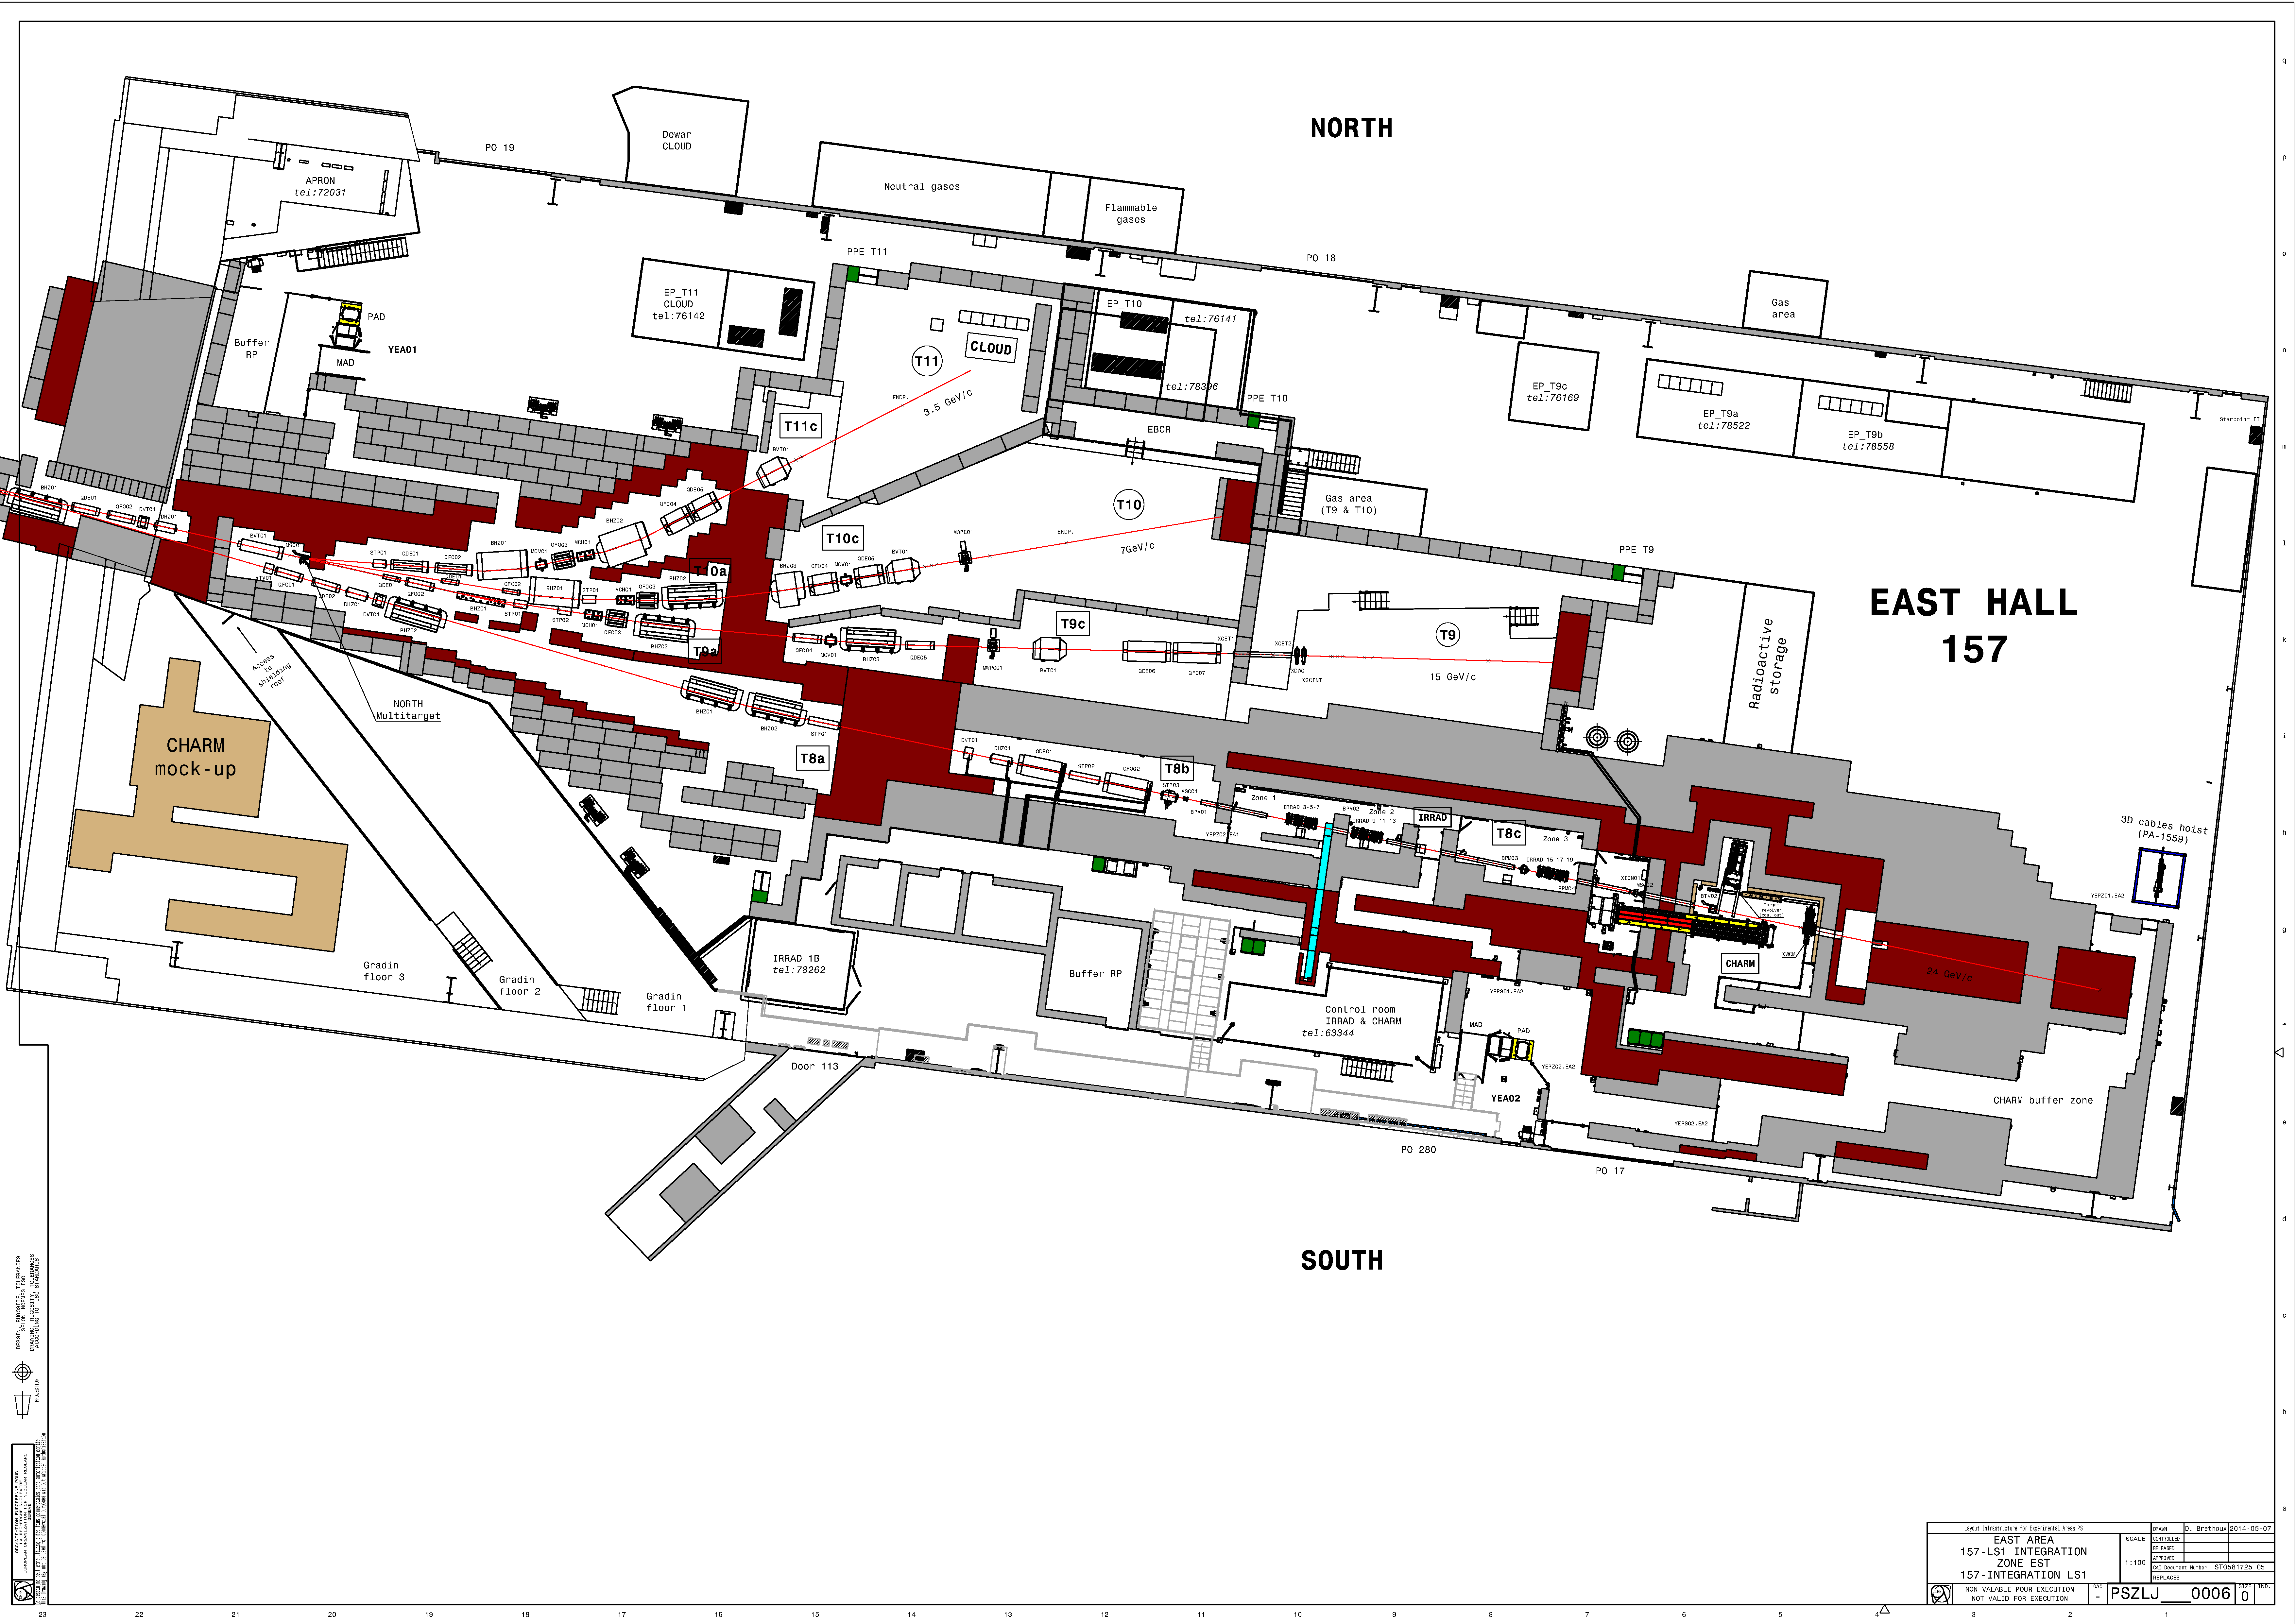
\includegraphics[width=\textwidth]{immagini/EastArea2014-final.pdf}
\caption{\small \it The East Area of the PS/SPS
  complex~\cite{cern_east}.}\label{fig:cern_east} %\url{http://sba.web.cern.ch/sba/BeamsAndAreas/East/}
\end{figure}
The beam delivered on the T9 beamline is the result of the interaction of the
primary beam, whose energy is 24 GeV, with a target to produce a secondary
beam. The resulting beam, composed of electron, muons and hadrons has in the
range 0.5 to 15 GeV. Typical intensities are of the order of 10$^4$-10$^6$ particles
per spill, each spill being about 400 ms long. The spill repetition varies from a few
seconds to $\sim$40 seconds.\\
The experimental area contains a number of fixed detectors along with devices
that can be changed or added. Among the devices:
\begin{itemize}
\item different target are available, allowing different components of the
  beam. The core of the target is always light material;
\item two collimators filter the beam. A horizontal collimator changes the
  width of the momentum distribution of the beam rejecting particles that have
  either a higher or lower momentum with respect a given interval. A vertical
  collimator filters particles according to their initial angle on leaving the
  target;
\item a dipole magnet whose field can be varied allows to determine the momentum
  of the particles;
\item bending magnets are used in the beamline to guide the particles in a
  certain direction and to select the particles energies;
\item quadrupole magnets are used to control the beam size and to focus or
  defocus the particles in the beam line;
\item two Cherenkov counters allows to identify particles depending on the
  choice of gas and its pressure.
\end{itemize}
The combination of collimators and magnets allows to set the momentum resolution
in steps of 1\%$\frac{\Delta p}{p}$~\cite{muller2001optics}. The beam dimension
can be tuned using the secondary collimators and the quadrupole magnets,
obtaining values of the order of a few centimeters RMS, with a typical beam
divergence of $\sim$1 mrad.

